\documentclass[a4paper,conference,onecolumn]{IEEEtran}
\IEEEoverridecommandlockouts
\usepackage{wwpaper}
\usepackage{graphicx}
\hyphenation{op-tical net-works semi-conduc-tor}
\renewcommand{\subsection}[1]{%
  \vspace{\lineskip}%
  \begin{center}%
    \textit{#1}%
  \end{center}%
  \vspace{\lineskip}%
}

\begin{document}
\title{High-speed Universal Broadband for Scotland}
\author{
  \IEEEauthorblockN{%
    Peter Buneman\\ and Michael Fourman
  }
  \IEEEauthorblockA{%
    School of Informatics\\
    University of Edinburgh
  }
  \and
  \IEEEauthorblockN{%
    Marwan Fayed\\ and William Waites
  }
  \IEEEauthorblockA{%
    Dept. of Mathematics and Computing Science\\
    University of Stirling
  }
}
\IEEEspecialpapernotice{(bis)}
\maketitle

\begin{abstract}
  The HUBS project began with a small grant from the Carnegie
  Foundation to provide support for community networking initiatives in
  Scotland. It has been successful in the expansion and development of a
  group of pre-existing physically adjacent networks on the West Coast
  and assistance with the launch of new networks in Stirlingshire and
  Lanarkshire through sharing of expertise and loan of
  equipment. Importantly, several key areas have been identified where
  further work and longer term organisational effort are required --
  much remains to be done. This note outlines what has been
  accomplished so far and outlines a plan for the future to ensure 
  the long-term sustainability and continuing development of these
  initiatives.
\end{abstract}
\IEEEpeerreviewmaketitle

\section{Introduction}

The geography of Scotland presents some unique challenges for the
provisioning of high-speed internet access infrastructure to the
entire population. The mountainous terrain and sparse population mean
that methods of delivering service that require a certain density of
users and the corresponding economies of scale in order to be
profitable are not feasible in much of the country. This means
that in many places if Internet access is available from the ``usual
suspects'' the available capacity is small and hence the performance
is poor, and the obvious alternatives such as satellite are
exceptionally expensive and the performance is likewise poor.

This state of affairs has led communities in some parts of the
country to construct their own networks with very high capacity in the
local area and then to arrange to connect these networks to a place
where sufficient infrastructure exists to be able to connect with
other Internet service providers. These community networks effectively
become small-scale Internet service providers in their own right --
although their small size poses some challenges that the HUBS project
is well placed to help with.

\subsection{Tegola, Knoydart and the Small Isles}

The current work of the HUBS project began with taking stock of the
Tegola network which began as a University of Edinburgh research
project around Loch Hourn. Because of the collaboration of the
University of the Highlands and Islands, this network had access to
good bandwidth at the Sabhal Mòr Ostaig college on Skye and a wireless
network was constructed to distribute access to the settlements around
the loch. As the communities began to rely on the network, with some
people going so far as to use it as their only means of long-distance
communication throwing away their telephones, there was a need to
improve the robustness of the facilities as occasionally experiments
necessary for the research purposes proved disruptive to the service
delivered. 

Meanwhile, the communities on Knoydart and the Small Isles began, with
the assistance and advice of some of the people who had constructed
the Tegola network, to construct their own distribution
infrastructure on a similar model. Rather than connecting to the
academic backbone for upstream bandwidth, they purchased consumer-grade
DSL service at Mallaig and Arisaig and extended their networks to
those towns. The way this was done posed some technical
problems\footnote{See \textsc{Appendix \ref{sec:dsl}} for technical
  details} in terms of both capacity and resiliency in the face of
faults that occur from time to time either on the network itself or
upstream, outwith the direct control of the communities.

Because of the physical adjacency of these four networks\footnote{See
  diagram \textsc{Appendix \ref{sec:wcn}}} it made sense to interconnect
them so that regional traffic could remain in the region instead of
going to London and back, and, perhaps more importantly, each could
make use of the others' upstream connections in case theirs developed
a fault. Doing this properly, in such a way that each network
maintains its autonomy in terms of internal architecture and
management, involved using techniques that are normally used by
Internet service providers and some large private networks such as
Ja.net. This has been accomplished to an acceptable standard but has
been hampered by a lack of access to some specific types of resources
due to the small size of the individual organisations. This point, and
what can be done to smooth the process, is further elaborated below.

\subsection{Allanton}

Our work so far has not, however, been limited to working with already
existing community networks in advanced stages of development. In the
area near Allanton, South Lanarkshire, for example, are a dozen or so
farms that are too far from the nearest central office for DSL to be
available to them at any but the lowest possible speeds and there are
no plans on the part of any of the major carriers to rectify the
situation -- the cluster of farms represent too little potential
income to warrant what, for them, would be a significant investment in
infrastructure.

Many of these farms have, however, a good line of sight
to a particular church in the town that happens to be very near to the
fibre plant of one major carrier. We therefore loaned them some
wireless equipment, so that they could be satisfied that such things
do indeed work as they claim without any initial investment other than
a bit of their time, helped them configure it and also assisted with
negotiations with the church and said major carrier.

Our demonstrable experience with similar projects turns out to be very
useful when explaining to landowners what it is that the community
intends to do -- since in the initial stages a lack of experience on
the part of a the community means that they may need assistance in
articulating the details of their plan. Similarly, knowing exactly
what to ask for and using contacts that we already have with large
telecommunications carriers smoothes the process significantly,
cutting through marketing terms and helping to make sure that the
community is able to get what they require -- as opposed to what a
retail sales department may wish to sell them.

By far the most useful and yet simplest thing that we can do to help
initiatives that are just beginning is by having a pool of equipment
that can be lent out. The costs to build local infrastructure are not
great, but they can run into several hundred or some thousands of
pounds depending on the scope. If the communities -- who in many cases
have had organisations in the past come to them claiming to be able
deliver Internet service to them -- are not certain that it will work,
they will have trouble raising even this small amount of money. So if
they have access to the equipment initially and are able to
\textit{convince themselves}, then they are very likely to begin to
invest themselves. Without a facility like this, the barrier is simply
too high.

The network around Allanton is on track to go live in early to mid
November 2012.

\subsection{Blairlogie and Sherrifmuir}

Blairlogie, just to the East of the University of Stirling campus is
in a very similar situation to Allanton. The main difference being its
proximity to the university and hence the academic
network. Geographical features (specifically, trees) mean that a
direct connection to the university is not possible and a relay must
be used. Several good candidate sites have been identified and
negotiations are proceeding apace.

Sherrifmuir to the North of the university is almost an identical
situation save that a different geographical feature (mountain)
prevents connecting to the academic backbone. The nearby town of
Dunblane has, however, a well developed network infrastructure and
surveys are under way to identify suitable sites for interconnection
and a relay.

\subsection{Instructional and Educational Materials}

Throughout the project we have attempted to document our experiences. 
This has included both informal writings and progress updates,
essentially ``blog posts'' as well as more purposefully written
``howto'' documents. There is a substantial amount of accumulated
knowledge that has been gained in the course of this work that new
community infrastructure projects that are just starting out ought to
benefit from. It is difficult to distil this information down to
exactly what is required because each situation is different, and in
different ways. The local geography may differ, the skill-sets
available in the community may differ, as may levels of involvement or
commitment, and budgets, and tolerances for service interruptions or
degradation.

As we encounter different situations and craft different solutions,
what has seemed most relevant has been written down on the Tegola web
site\footnote{\url{http://www.tegola.org.uk/}} in the hope that it
might be of some use. We have tried so far as possible to keep the
material focused enough, in particular the ``howto'' manuals, that
someone who visits the web site in order to find out how to do a
particular, specific thing, is able to find the information that they
need, in a succinct and intelligable form. Already some feedback we
have received indicates that the material we have produced is at least
useful if not yet comprehensive. 

\newpage
\section{The Evolution of HUBS}

\subsection{Loan of Equipment}
\subsection{Economies of Scale}
\subsection{Developmental Support}
\subsection{Operational Support}
\subsection{Coordination}

\newpage{Staffing and Finance}

\begin{appendices}
  \newpage
  \section{Consumer-grade DSL}
  \label{sec:dsl}

  \newpage
  \section{Network Numbers}
  \label{sec:numbers}

  \newpage
  \section{West Coast Networks}
  \label{sec:wcn}
  \vspace{24pt}
  \begin{center}
    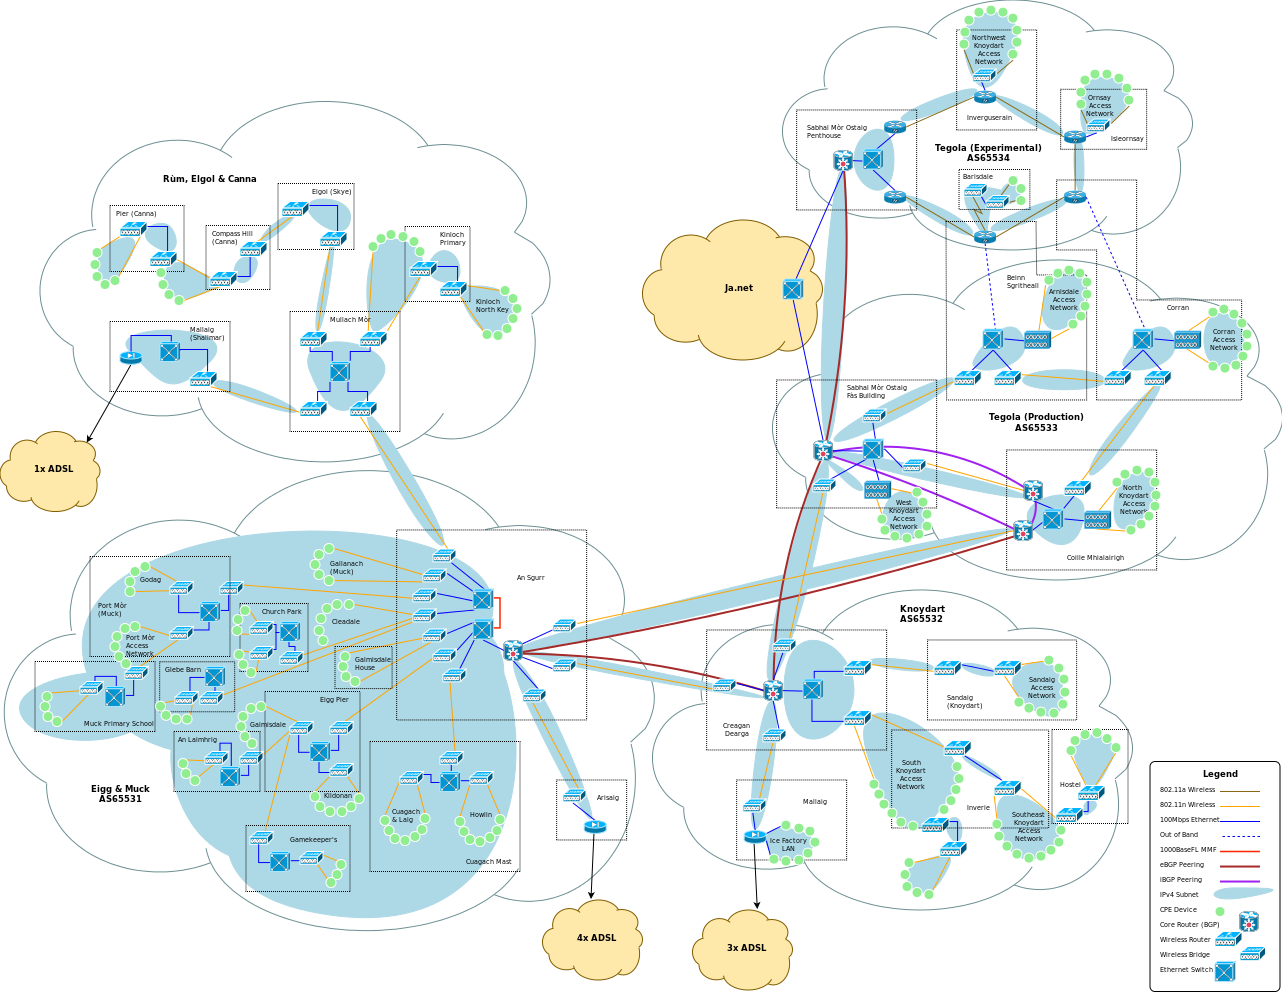
\includegraphics[scale=0.35,angle=270]{../diagrams/west-coast-detail.eps}
  \end{center}
\end{appendices}

\end{document}


